\documentclass{article}
\usepackage[dvipsnames]{xcolor}
\usepackage{calc}
\usepackage{fancybox}
\usepackage{tikz}
\usepackage{mathptmx}
\usepackage[11pt]{moresize}
\usetikzlibrary{positioning}
\usetikzlibrary{shapes,snakes}
\usepackage{amsmath,amssymb}
\begin{document}
\title{Project K Tools}
\maketitle
\author{\textit{S\^{a}rbu Iulia Iustina, grupa B1}}
\newline
\newline
\textit{Syntax}\newline

 \qquad The K syntax of languages, calculi or systems, as well as the additional syntax needed for the semantics of these, is defined using context-free grammars (CFG) or, equivalently, algebraic signatures written using the mixfix notation (i.e., operation names include underscores as argument placeholders) [ 23 ,22,12]. We take the freedom to borrow from the algebraic universe any structures of interest on a by-need basis.  In this paper we use \textit{List\{Nonterminal,terminal\}} to refer to the nonterminal corresponding to \textit{terminal}-separated lists of \textit{Non-terminal}elements; for example,\textit{List\{Exp,@\}}stands for \textit{@}-separated lists of expressions. We skip the terminal when it is a comma; e.g.,\textit{List\{Exp\}}stands for comma-separated lists of expressions.\newline\newline
module IMP-SYNTAX
\newline
\newline

\textit{Expressions}
\newline

 \qquad The syntax of expressions is identical to that in untyped SIMPLE, except for  the  logical  conjunction  and  disjunction  which  have  different  strictness attributes, because they now have different evaluation strategies.\newline\newline
syntax AExp ::=  Int  (  builtin ) 


 
\hspace{35pt} \qquad $\arrowvert$  Id  (  builtin ) 


 
\hspace{35pt} \qquad $\arrowvert$  String  (  builtin ) 


 
\hspace{35pt} \qquad $\arrowvert$ 
"read"
"(" ")"

 
\hspace{35pt} \qquad $\arrowvert$ 
"++" Id 

\hspace{35pt} \qquad $>$ left: 

\hspace{35pt} \qquad  AExp 
"*" AExp 
[left]

 
\hspace{35pt} \qquad $\arrowvert$  AExp 
"/" AExp 
[left]

\hspace{35pt} \qquad $>$ left: 

\hspace{35pt} \qquad  AExp 
"+" AExp 
[left, strict]

 
\hspace{35pt} \qquad $\arrowvert$  AExp 
"-" AExp 
[left]

 
\hspace{35pt} \qquad $\arrowvert$ 
"(" AExp ")"
[bracket]
\newline
syntax BExp ::=  Bool  (  builtin ) 


 
\hspace{35pt} \qquad $\arrowvert$ "!" BExp 

 
\hspace{35pt} \qquad $\arrowvert$  BExp 
 "\&\&"  BExp 
[non-assoc]

 
\hspace{35pt} \qquad $\arrowvert$  AExp 
 "$<=$"  AExp 
[strict]

 
\hspace{35pt} \qquad $\arrowvert$  AExp 
 "$<$"  AExp 

 
\hspace{35pt} \qquad $\arrowvert$ 
"(" BExp ")"
[bracket]
\newline

\textit{Statements}
\newline

 \qquad The statements have the same syntax as in untyped SIMPLE, except for the exceptions, which now type their parameter.  Unlike in untyped SIMPLE, all statement constructs which have arguments and are not desugared are strict, including the conditional and the while. Indeed, from a typing perspective,they are all strict: first type their arguments and then type the actual construct.\newline\newline
syntax Block ::=  "\{"  Stmt 
 "\}" 

 
\hspace{35pt} \qquad $\arrowvert$ 
 "\{" 
 "\}" 
\newline
syntax Stmt ::=  Block 
 
\hspace{35pt} \qquad $\arrowvert$ "int" Id 
";"

 
\hspace{35pt} \qquad $\arrowvert$ 
"print"
"(" AExp ")"
";"
[strict]

 
\hspace{35pt} \qquad $\arrowvert$  Id 
"=" AExp 
";"
[strict(2)]

 
\hspace{35pt} \qquad $\arrowvert$ 
"if" BExp 
 Block 
"else" Block 
[strict(1)]

 
\hspace{35pt} \qquad $\arrowvert$ 
"while" BExp 
 Block 

\hspace{35pt} \qquad $>$  Stmt 
 Stmt 
[right]
\newline\newline
\textit{Static semantics}
\newline

\qquad Here we define the type system of SIMPLE. Like concrete semantics, type systems defined in K are also executable.  However,K type systems turn into type checkers instead of interpreters when executed. The typing process is done in two (overlapping) phases.  In the first phase the global environment is built, which contains type bindings for all the globally declared variables and functions.  For functions, the declared types will be \textit{trusted} during  the  first  phase  and  simply  bound  to  their  corresponding function names and placed in the global type environment.  At the same time, type-checking tasks that the function bodies indeed respect their claimed types are generated.  All these tasks are verified during the second phase.  This way, all the global variable and function declarations are available in the global type environment and can be used to type-check each function body.  This is consistent with the semantics of untyped SIMPLE, where functions can access all the global variables and can call any other function declared in the same program.  The two phases may overlap because of the K concurrent semantics. For example, a function task can be started while the first phase is still running; moreover, it may even complete before the first phase does, namely when all the global variables and functions that it needs have already been processed and made available in the global environment by the first phase task.\newline\newline
\newline 
 \newline 
module IMP
\newline
imports IMP-SYNTAX
\newline
\newline
\newline
\newline
syntax KResult ::=  Bool 
 
\hspace{35pt} \qquad $\arrowvert$  Int 

 
\hspace{35pt} \qquad $\arrowvert$  String 
\newline\newline

\textit{Configuration}
\newline

 \qquad The configuration of our type system consists of a tasks cell holding various typing task cells, and a global type environment.\newline\newline
\newline\newline
\textit{CONFIGURATION: }
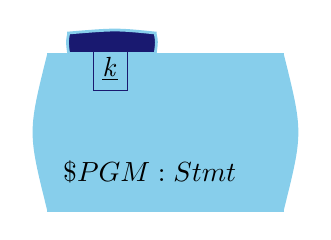
\begin{tikzpicture}\fill[color=SkyBlue] (0,0) rectangle (3,2);
\draw[color=SkyBlue] (0,0) rectangle (3,2); 
\fill[color=SkyBlue] (3,0).. controls (3.25,1).. (3,2) -- (3,0);
\fill[color=SkyBlue] (0,0).. controls (-0.25,1).. (0,2) -- (0,0);
\fill[color=MidnightBlue] (0.27,2).. controls (0.25,2.15).. (0.27,2.25)--(0.27,2.26).. controls(0.87,2.31).. (1.37,2.26)--(1.37,2.25).. controls(1.39,2.15).. (1.37,2)--(0.27,2);
\draw[color=SkyBlue,line width=1pt] (0.27,2).. controls (0.25,2.15).. (0.27,2.25)--(0.27,2.26).. controls(0.87,2.31).. (1.37,2.26)--(1.37,2.25).. controls(1.39,2.15).. (1.37,2)--(0.27,2);
\node[draw=SkyBlue] at (1.3,0.5) 
{$\$PGM: Stmt$};
\node[draw=MidnightBlue] at (0.8,1.8)
{\underline{\textit{k}}};
\end{tikzpicture}
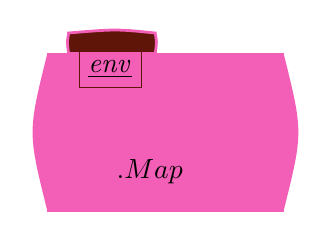
\begin{tikzpicture}\fill[color=CarnationPink] (0,0) rectangle (3,2);
\draw[color=CarnationPink] (0,0) rectangle (3,2); 
\fill[color=CarnationPink] (3,0).. controls (3.25,1).. (3,2) -- (3,0);
\fill[color=CarnationPink] (0,0).. controls (-0.25,1).. (0,2) -- (0,0);
\fill[color=Sepia] (0.27,2).. controls (0.25,2.15).. (0.27,2.25)--(0.27,2.26).. controls(0.87,2.31).. (1.37,2.26)--(1.37,2.25).. controls(1.39,2.15).. (1.37,2)--(0.27,2);
\draw[color=CarnationPink,line width=1pt] (0.27,2).. controls (0.25,2.15).. (0.27,2.25)--(0.27,2.26).. controls(0.87,2.31).. (1.37,2.26)--(1.37,2.25).. controls(1.39,2.15).. (1.37,2)--(0.27,2);
\node[draw=CarnationPink] at (1.3,0.5) 
{$.Map$};
\node[draw=Sepia] at (0.8,1.8)
{\underline{\textit{env}}};
\end{tikzpicture}
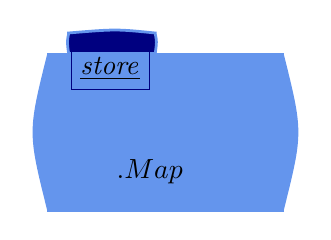
\begin{tikzpicture}\fill[color=CornflowerBlue] (0,0) rectangle (3,2);
\draw[color=CornflowerBlue] (0,0) rectangle (3,2); 
\fill[color=CornflowerBlue] (3,0).. controls (3.25,1).. (3,2) -- (3,0);
\fill[color=CornflowerBlue] (0,0).. controls (-0.25,1).. (0,2) -- (0,0);
\fill[color=NavyBlue] (0.27,2).. controls (0.25,2.15).. (0.27,2.25)--(0.27,2.26).. controls(0.87,2.31).. (1.37,2.26)--(1.37,2.25).. controls(1.39,2.15).. (1.37,2)--(0.27,2);
\draw[color=CornflowerBlue,line width=1pt] (0.27,2).. controls (0.25,2.15).. (0.27,2.25)--(0.27,2.26).. controls(0.87,2.31).. (1.37,2.26)--(1.37,2.25).. controls(1.39,2.15).. (1.37,2)--(0.27,2);
\node[draw=CornflowerBlue] at (1.3,0.5) 
{$.Map$};
\node[draw=NavyBlue] at (0.8,1.8)
{\underline{\textit{store}}};
\end{tikzpicture}
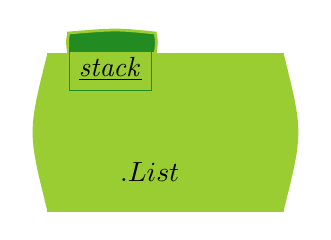
\begin{tikzpicture}\fill[color=YellowGreen] (0,0) rectangle (3,2);
\draw[color=YellowGreen] (0,0) rectangle (3,2); 
\fill[color=YellowGreen] (3,0).. controls (3.25,1).. (3,2) -- (3,0);
\fill[color=YellowGreen] (0,0).. controls (-0.25,1).. (0,2) -- (0,0);
\fill[color=ForestGreen] (0.27,2).. controls (0.25,2.15).. (0.27,2.25)--(0.27,2.26).. controls(0.87,2.31).. (1.37,2.26)--(1.37,2.25).. controls(1.39,2.15).. (1.37,2)--(0.27,2);
\draw[color=YellowGreen,line width=1pt] (0.27,2).. controls (0.25,2.15).. (0.27,2.25)--(0.27,2.26).. controls(0.87,2.31).. (1.37,2.26)--(1.37,2.25).. controls(1.39,2.15).. (1.37,2)--(0.27,2);
\node[draw=YellowGreen] at (1.3,0.5) 
{$.List$};
\node[draw=ForestGreen] at (0.8,1.8)
{\underline{\textit{stack}}};
\end{tikzpicture}
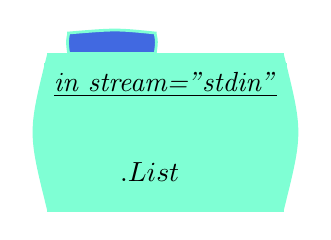
\begin{tikzpicture}\fill[color=Aquamarine] (0,0) rectangle (3,2);
\draw[color=Aquamarine] (0,0) rectangle (3,2); 
\fill[color=Aquamarine] (3,0).. controls (3.25,1).. (3,2) -- (3,0);
\fill[color=Aquamarine] (0,0).. controls (-0.25,1).. (0,2) -- (0,0);
\fill[color=RoyalBlue] (0.27,2).. controls (0.25,2.15).. (0.27,2.25)--(0.27,2.26).. controls(0.87,2.31).. (1.37,2.26)--(1.37,2.25).. controls(1.39,2.15).. (1.37,2)--(0.27,2);
\draw[color=Aquamarine,line width=1pt] (0.27,2).. controls (0.25,2.15).. (0.27,2.25)--(0.27,2.26).. controls(0.87,2.31).. (1.37,2.26)--(1.37,2.25).. controls(1.39,2.15).. (1.37,2)--(0.27,2);
\node[draw=Aquamarine] at (1.3,0.5) 
{$.List$};
\node[draw=Aquamarine] at (1.5,1.6)
{\underline{\textit{in stream="stdin"}}};
\end{tikzpicture}
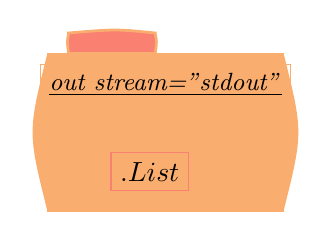
\begin{tikzpicture}\fill[color=Apricot] (0,0) rectangle (3,2);
\draw[color=Apricot] (0,0) rectangle (3,2); 
\fill[color=Apricot] (3,0).. controls (3.25,1).. (3,2) -- (3,0);
\fill[color=Apricot] (0,0).. controls (-0.25,1).. (0,2) -- (0,0);
\fill[color=Salmon] (0.27,2).. controls (0.25,2.15).. (0.27,2.25)--(0.27,2.26).. controls(0.87,2.31).. (1.37,2.26)--(1.37,2.25).. controls(1.39,2.15).. (1.37,2)--(0.27,2);
\draw[color=Apricot,line width=1pt] (0.27,2).. controls (0.25,2.15).. (0.27,2.25)--(0.27,2.26).. controls(0.87,2.31).. (1.37,2.26)--(1.37,2.25).. controls(1.39,2.15).. (1.37,2)--(0.27,2);
\node[draw=Salmon] at (1.3,0.5) 
{$.List$};
\node[draw=Apricot] at (1.5,1.6)
{\underline{\textit{\small out stream="stdout"}}};
\end{tikzpicture}\newline\newline\newline\newline\newline

\textit{Common expression constructs}
\newline

 \qquad The rules below are straightforward and self-explanatory:\newline\newline

\noindent\fcolorbox{Black}{White}{\parbox{3in}{RULE \newline I1 $int$ $<=$ I2 $int$ $=>$ I1 $<=int$ I2 }}
\noindent\fcolorbox{Black}{White}{\parbox{3in}{RULE \newline I1 $int$ $+$ I2 $int$ $=>$ I1 $+int$ I2 }}
\noindent\fcolorbox{Black}{White}{\parbox{3in}{RULE \newline S1 $stmt$ S2 $stmt$ $=>$ S1 $\sim>$ S2 }}
\newline\newline\newline
\noindent\fcolorbox{Black}{White}{\parbox{2in}{RULE 
\newline\newline\newline
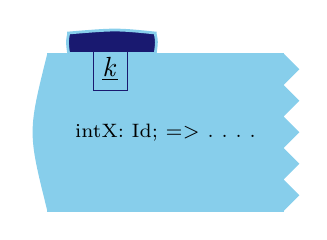
\begin{tikzpicture}
\fill[color=SkyBlue] (0,0) rectangle (3,2);
\draw[color=SkyBlue] (0,0) rectangle (3,2); 
\fill[color=SkyBlue] (3,0) -- (3.2,0.2) -- (3,0.4) -- (3.2,0.6) -- (3,0.8) -- (3.2,1) -- (3,1.2) -- (3.2,1.4)--(3,1.6)--(3.2,1.8)--(3,2)--(3,0);
\fill[color=SkyBlue] (0,0).. controls (-0.25,1).. (0,2) -- (0,0);
\fill[color=MidnightBlue] (0.27,2).. controls (0.25,2.15).. (0.27,2.25)--(0.27,2.26).. controls(0.87,2.31).. (1.37,2.26)--(1.37,2.25).. controls(1.39,2.15).. (1.37,2)--(0.27,2);
\draw[color=SkyBlue,line width=1pt] (0.27,2).. controls (0.25,2.15).. (0.27,2.25)--(0.27,2.26).. controls(0.87,2.31).. (1.37,2.26)--(1.37,2.25).. controls(1.39,2.15).. (1.37,2)--(0.27,2);
\node[draw=MidnightBlue] at (0.8,1.8){\underline{\textit{k}}};
\node[draw=SkyBlue] at (1.5,1) {\ssmall intX$:$ Id$;$ $=>$ $.$ $.$ $.$ $.$ };
\end{tikzpicture}
\newline\newline
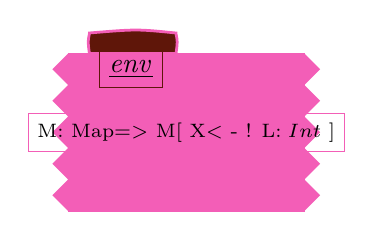
\begin{tikzpicture}
\fill[color=CarnationPink] (0,0) rectangle (3,2);
\draw[color=CarnationPink] (0,0) rectangle (3,2); 
\fill[color=CarnationPink] (3,0) -- (3.2,0.2) -- (3,0.4) -- (3.2,0.6) -- (3,0.8) -- (3.2,1) -- (3,1.2) -- (3.2,1.4)--(3,1.6)--(3.2,1.8)--(3,2)--(3,0);
\fill[color=CarnationPink] (0,0) -- (-0.2,0.2) -- (0,0.4) -- (-0.2,0.6) -- (0,0.8) -- (-0.2,1) -- (0,1.2) -- (-0.2,1.4)--(0,1.6)--(-0.2,1.8)--(0,2)--(0,0);
\fill[color=Sepia] (0.27,2).. controls (0.25,2.15).. (0.27,2.25)--(0.27,2.26).. controls(0.87,2.31).. (1.37,2.26)--(1.37,2.25).. controls(1.39,2.15).. (1.37,2)--(0.27,2);
\draw[color=CarnationPink,line width=1pt] (0.27,2).. controls (0.25,2.15).. (0.27,2.25)--(0.27,2.26).. controls(0.87,2.31).. (1.37,2.26)--(1.37,2.25).. controls(1.39,2.15).. (1.37,2)--(0.27,2);
\node[draw=Sepia] at (0.8,1.8){\underline{\textit{env}}};
\node[draw=CarnationPink] at (1.5,1) {\ssmall M$:$ Map$=>$ M$[$ X$<$ - ! L$:Int$ $]$ };
\end{tikzpicture}
\newline\newline
\begin{tikzpicture}
\fill[color=CornflowerBlue] (0,0) rectangle (3,2);
\draw[color=CornflowerBlue] (0,0) rectangle (3,2); 
\fill[color=CornflowerBlue] (3,0).. controls (3.25,1).. (3,2) -- (3,0);
\fill[color=CornflowerBlue] (0,0).. controls (-0.25,1).. (0,2) -- (0,0);
\fill[color=NavyBLue] (0.27,2).. controls (0.25,2.15).. (0.27,2.25)--(0.27,2.26).. controls(0.87,2.31).. (1.37,2.26)--(1.37,2.25).. controls(1.39,2.15).. (1.37,2)--(0.27,2);
\draw[color=CornflowerBlue,line width=1pt] (0.27,2).. controls (0.25,2.15).. (0.27,2.25)--(0.27,2.26).. controls(0.87,2.31).. (1.37,2.26)--(1.37,2.25).. controls(1.39,2.15).. (1.37,2)--(0.27,2);
\node[draw=NavyBLue] at (0.8,1.8){\underline{\textit{store}}};
\node[draw=CornflowerBlue] at (1.5,1) {\ssmall M"$:$ Map$($ $.$ Map$=>$ ! L$|->$0$)$ };
\end{tikzpicture}}
}\newline
\newline\newline\newline
\noindent\fcolorbox{Black}{White}{\parbox{2in}{RULE 
\newline\newline\newline
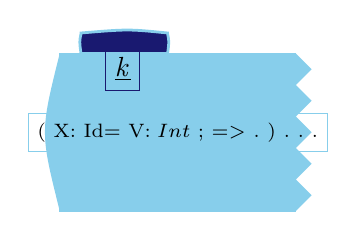
\begin{tikzpicture}
\fill[color=SkyBlue] (0,0) rectangle (3,2);
\draw[color=SkyBlue] (0,0) rectangle (3,2); 
\fill[color=SkyBlue] (3,0) -- (3.2,0.2) -- (3,0.4) -- (3.2,0.6) -- (3,0.8) -- (3.2,1) -- (3,1.2) -- (3.2,1.4)--(3,1.6)--(3.2,1.8)--(3,2)--(3,0);
\fill[color=SkyBlue] (0,0).. controls (-0.25,1).. (0,2) -- (0,0);
\fill[color=MidnightBlue] (0.27,2).. controls (0.25,2.15).. (0.27,2.25)--(0.27,2.26).. controls(0.87,2.31).. (1.37,2.26)--(1.37,2.25).. controls(1.39,2.15).. (1.37,2)--(0.27,2);
\draw[color=SkyBlue,line width=1pt] (0.27,2).. controls (0.25,2.15).. (0.27,2.25)--(0.27,2.26).. controls(0.87,2.31).. (1.37,2.26)--(1.37,2.25).. controls(1.39,2.15).. (1.37,2)--(0.27,2);
\node[draw=MidnightBlue] at (0.8,1.8){\underline{\textit{k}}};
\node[draw=SkyBlue] at (1.5,1) {\ssmall $($ X$:$ Id$=$ V$:Int$ $;$ $=>$ $.$ $)$ $.$ $.$ $.$ };
\end{tikzpicture}
\newline\newline
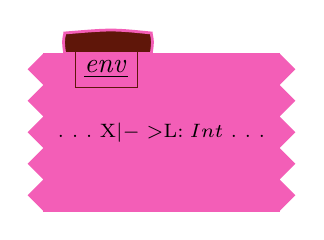
\begin{tikzpicture}
\fill[color=CarnationPink] (0,0) rectangle (3,2);
\draw[color=CarnationPink] (0,0) rectangle (3,2); 
\fill[color=CarnationPink] (3,0) -- (3.2,0.2) -- (3,0.4) -- (3.2,0.6) -- (3,0.8) -- (3.2,1) -- (3,1.2) -- (3.2,1.4)--(3,1.6)--(3.2,1.8)--(3,2)--(3,0);
\fill[color=CarnationPink] (0,0) -- (-0.2,0.2) -- (0,0.4) -- (-0.2,0.6) -- (0,0.8) -- (-0.2,1) -- (0,1.2) -- (-0.2,1.4)--(0,1.6)--(-0.2,1.8)--(0,2)--(0,0);
\fill[color=Sepia] (0.27,2).. controls (0.25,2.15).. (0.27,2.25)--(0.27,2.26).. controls(0.87,2.31).. (1.37,2.26)--(1.37,2.25).. controls(1.39,2.15).. (1.37,2)--(0.27,2);
\draw[color=CarnationPink,line width=1pt] (0.27,2).. controls (0.25,2.15).. (0.27,2.25)--(0.27,2.26).. controls(0.87,2.31).. (1.37,2.26)--(1.37,2.25).. controls(1.39,2.15).. (1.37,2)--(0.27,2);
\node[draw=Sepia] at (0.8,1.8){\underline{\textit{env}}};
\node[draw=CarnationPink] at (1.5,1) {\ssmall $.$ $.$ $.$ X$|->$L$:Int$ $.$ $.$ $.$ };
\end{tikzpicture}
\newline\newline
\begin{tikzpicture}
\fill[color=CornflowerBlue] (0,0) rectangle (3,2);
\draw[color=CornflowerBlue] (0,0) rectangle (3,2); 
\fill[color=CornflowerBlue] (3,0).. controls (3.25,1).. (3,2) -- (3,0);
\fill[color=CornflowerBlue] (0,0).. controls (-0.25,1).. (0,2) -- (0,0);
\fill[color=NavyBLue] (0.27,2).. controls (0.25,2.15).. (0.27,2.25)--(0.27,2.26).. controls(0.87,2.31).. (1.37,2.26)--(1.37,2.25).. controls(1.39,2.15).. (1.37,2)--(0.27,2);
\draw[color=CornflowerBlue,line width=1pt] (0.27,2).. controls (0.25,2.15).. (0.27,2.25)--(0.27,2.26).. controls(0.87,2.31).. (1.37,2.26)--(1.37,2.25).. controls(1.39,2.15).. (1.37,2)--(0.27,2);
\node[draw=NavyBLue] at (0.8,1.8){\underline{\textit{store}}};
\node[draw=CornflowerBlue] at (1.5,1) {\ssmall $.$ $.$ $.$ L$|->$$($ \_$=>$ V$)$ $.$ $.$ $.$ };
\end{tikzpicture}}
}\newline
\newline\newline\newline
\noindent\fcolorbox{Black}{White}{\parbox{2in}{RULE 
\newline\newline\newline
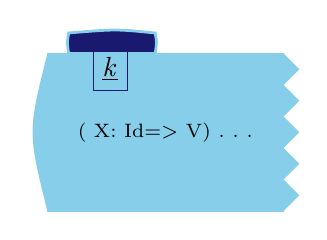
\begin{tikzpicture}
\fill[color=SkyBlue] (0,0) rectangle (3,2);
\draw[color=SkyBlue] (0,0) rectangle (3,2); 
\fill[color=SkyBlue] (3,0) -- (3.2,0.2) -- (3,0.4) -- (3.2,0.6) -- (3,0.8) -- (3.2,1) -- (3,1.2) -- (3.2,1.4)--(3,1.6)--(3.2,1.8)--(3,2)--(3,0);
\fill[color=SkyBlue] (0,0).. controls (-0.25,1).. (0,2) -- (0,0);
\fill[color=MidnightBlue] (0.27,2).. controls (0.25,2.15).. (0.27,2.25)--(0.27,2.26).. controls(0.87,2.31).. (1.37,2.26)--(1.37,2.25).. controls(1.39,2.15).. (1.37,2)--(0.27,2);
\draw[color=SkyBlue,line width=1pt] (0.27,2).. controls (0.25,2.15).. (0.27,2.25)--(0.27,2.26).. controls(0.87,2.31).. (1.37,2.26)--(1.37,2.25).. controls(1.39,2.15).. (1.37,2)--(0.27,2);
\node[draw=MidnightBlue] at (0.8,1.8){\underline{\textit{k}}};
\node[draw=SkyBlue] at (1.5,1) {\ssmall $($ X$:$ Id$=>$ V$)$ $.$ $.$ $.$ };
\end{tikzpicture}
\newline\newline
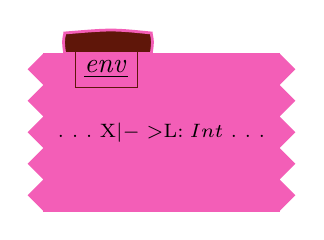
\begin{tikzpicture}
\fill[color=CarnationPink] (0,0) rectangle (3,2);
\draw[color=CarnationPink] (0,0) rectangle (3,2); 
\fill[color=CarnationPink] (3,0) -- (3.2,0.2) -- (3,0.4) -- (3.2,0.6) -- (3,0.8) -- (3.2,1) -- (3,1.2) -- (3.2,1.4)--(3,1.6)--(3.2,1.8)--(3,2)--(3,0);
\fill[color=CarnationPink] (0,0) -- (-0.2,0.2) -- (0,0.4) -- (-0.2,0.6) -- (0,0.8) -- (-0.2,1) -- (0,1.2) -- (-0.2,1.4)--(0,1.6)--(-0.2,1.8)--(0,2)--(0,0);
\fill[color=Sepia] (0.27,2).. controls (0.25,2.15).. (0.27,2.25)--(0.27,2.26).. controls(0.87,2.31).. (1.37,2.26)--(1.37,2.25).. controls(1.39,2.15).. (1.37,2)--(0.27,2);
\draw[color=CarnationPink,line width=1pt] (0.27,2).. controls (0.25,2.15).. (0.27,2.25)--(0.27,2.26).. controls(0.87,2.31).. (1.37,2.26)--(1.37,2.25).. controls(1.39,2.15).. (1.37,2)--(0.27,2);
\node[draw=Sepia] at (0.8,1.8){\underline{\textit{env}}};
\node[draw=CarnationPink] at (1.5,1) {\ssmall $.$ $.$ $.$ X$|->$L$:Int$ $.$ $.$ $.$ };
\end{tikzpicture}
\newline\newline
\begin{tikzpicture}
\fill[color=CornflowerBlue] (0,0) rectangle (3,2);
\draw[color=CornflowerBlue] (0,0) rectangle (3,2); 
\fill[color=CornflowerBlue] (3,0).. controls (3.25,1).. (3,2) -- (3,0);
\fill[color=CornflowerBlue] (0,0).. controls (-0.25,1).. (0,2) -- (0,0);
\fill[color=NavyBLue] (0.27,2).. controls (0.25,2.15).. (0.27,2.25)--(0.27,2.26).. controls(0.87,2.31).. (1.37,2.26)--(1.37,2.25).. controls(1.39,2.15).. (1.37,2)--(0.27,2);
\draw[color=CornflowerBlue,line width=1pt] (0.27,2).. controls (0.25,2.15).. (0.27,2.25)--(0.27,2.26).. controls(0.87,2.31).. (1.37,2.26)--(1.37,2.25).. controls(1.39,2.15).. (1.37,2)--(0.27,2);
\node[draw=NavyBLue] at (0.8,1.8){\underline{\textit{store}}};
\node[draw=CornflowerBlue] at (1.5,1) {\ssmall $.$ $.$ $.$ L$|->$V$:Int$ $.$ $.$ $.$ };
\end{tikzpicture}}
}\newline
\noindent\fcolorbox{Black}{White}{\parbox{3in}{RULE \newline IF true B1 $block$ else B2 $block$ $=>$ B1 }}
\noindent\fcolorbox{Black}{White}{\parbox{3in}{RULE \newline IF false B1 $block$ else B2 $block$ $=>$ B2 }}\newline
\newline
\newline
syntax KItem ::= "restoreEnv"
\noindent\fcolorbox{Black}{White}{\parbox{3in}{RULE \newline $\{$ $\}$ $=>$ $.$ }}
\noindent\fcolorbox{Black}{White}{\parbox{3in}{RULE \newline WHILE  $BExp$ $\{$  $stmt$ $\}$ $=>$ IF  $\{$  WHILE  $\{$  $\}$ $\}$ else $\{$ $\}$ }}\newline\newline

\textit{Conclusion}
\newline

 \qquad The K semantic framework,  consisting of a general-purpose concurrent rewriting approach together with a definitional technique specialized for con-current programming languages and systems, brings together the advantages of existing language definitional frameworks while avoiding their limitations. In spite of its youth, the K framework has already proven to be practical, as it has been used with relatively little effort to define complex languages like Java, Scheme, Verilog, or C, and to use those definitions for analyzing programs written in those languages. K is currently under heavy development, with bugs being fixed and new features and capabilities added on a regular basis.\newline\newline

\end{document}
